\documentclass[11pt]{article}
\usepackage[UTF8]{ctex}
\usepackage{indentfirst}
%\setlength{\parindent}{2em}

% some package

% graph
\RequirePackage{graphicx}
\RequirePackage{subfigure}
\RequirePackage{float}
% math
\RequirePackage{amsmath}
\RequirePackage{amssymb,amsfonts,mathrsfs}

\RequirePackage{bm}         % \mathbf{}
\RequirePackage{color}      % the color of the font
\usepackage{mathrsfs}
\RequirePackage{enumerate}

% like word
\usepackage[top=2.54cm, bottom=2.54cm, left=3.17cm, right=3.17cm]{geometry}


%\usefonttheme{professionalfonts}

% the caption of thf figure
\renewcommand{\figurename}{图}


\title{ \textbf{生物智能课程论文-复杂网络基础} }


\author{
	赵帅  \qquad 计算机学院  \qquad 21721043\\
	21721043@zju.edu.cn
}

\date{ }

\begin{document}
	
	\maketitle
	\section{什么是复杂网络}
		要研究复杂网络,首先要搞清楚复杂网络的定义。\par
		在网络理论的研究中,复杂网络是由数量巨大的节点和节点之间错综复杂的关系共同构成的网络结构。 \par
		用数学的语言来说,就是一个有着足够复杂的拓扑结构特征的图。\par
		复杂网络具有简单网络,如晶格网络、随机图等结构所不具备的特性,而这些特性往往出现在真实世界的网络结构中。\par
		复杂网络的研究是现今科学研究中的一个热点,与现实中各类高复杂性系统,如WWW、神经网络和社会网络~\cite{paper_01}的研究有密切关系。 \par
		我们也可以根据一些具体的特性来定义复杂网络:具有自组织、自相似、吸引子、小世界、无标度中部分或全部性质的网络称为复杂网络。这些特性我们在后面的文章中会详细解释。 \par
		下图是复杂网络的两个例子:
		
		\begin{figure}[htbp]
			\centering
			\begin{minipage}[t]{0.45\textwidth}
				\centering
				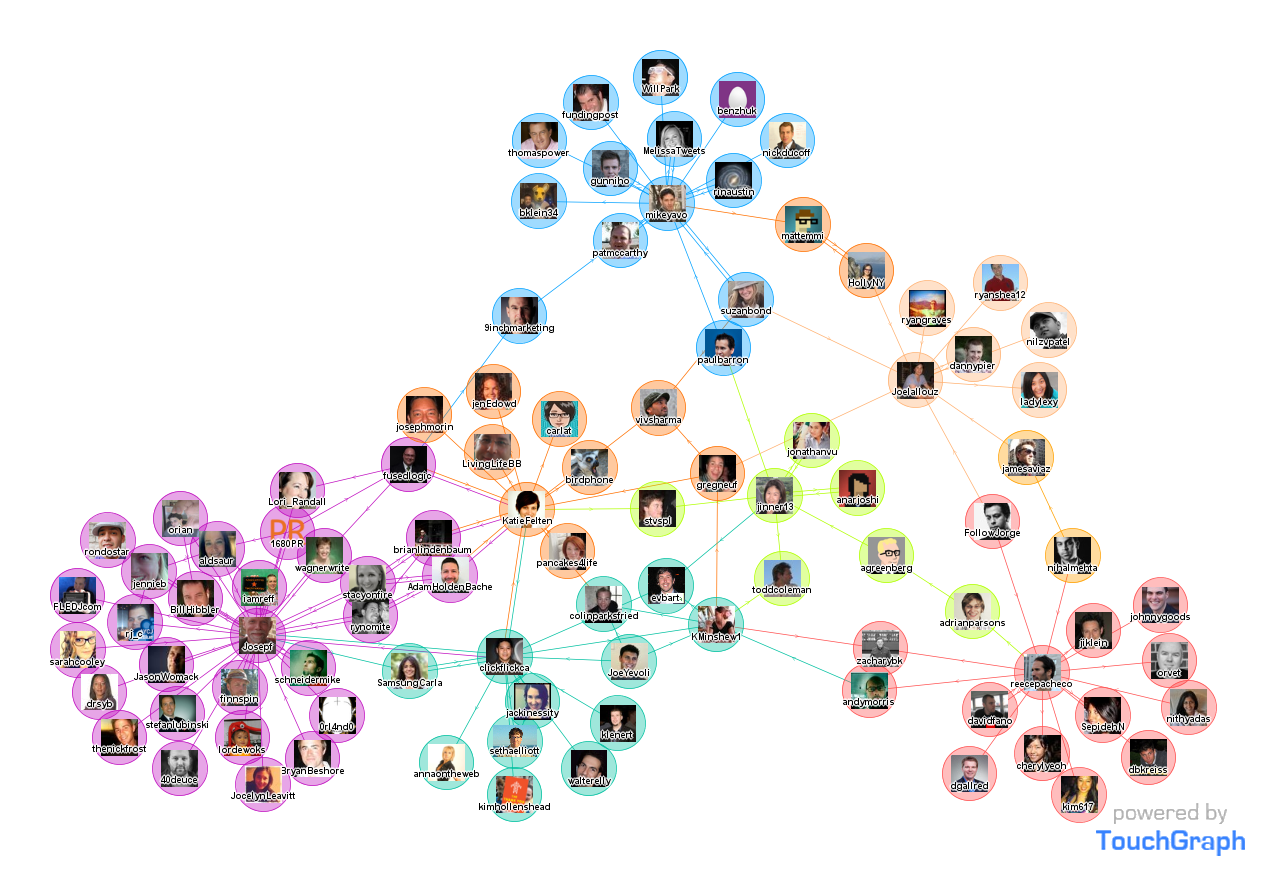
\includegraphics[height=4cm]{pic/01-social.png}
				\caption{社交网络}
			\end{minipage}
			\begin{minipage}[t]{0.45\textwidth}
				\centering
				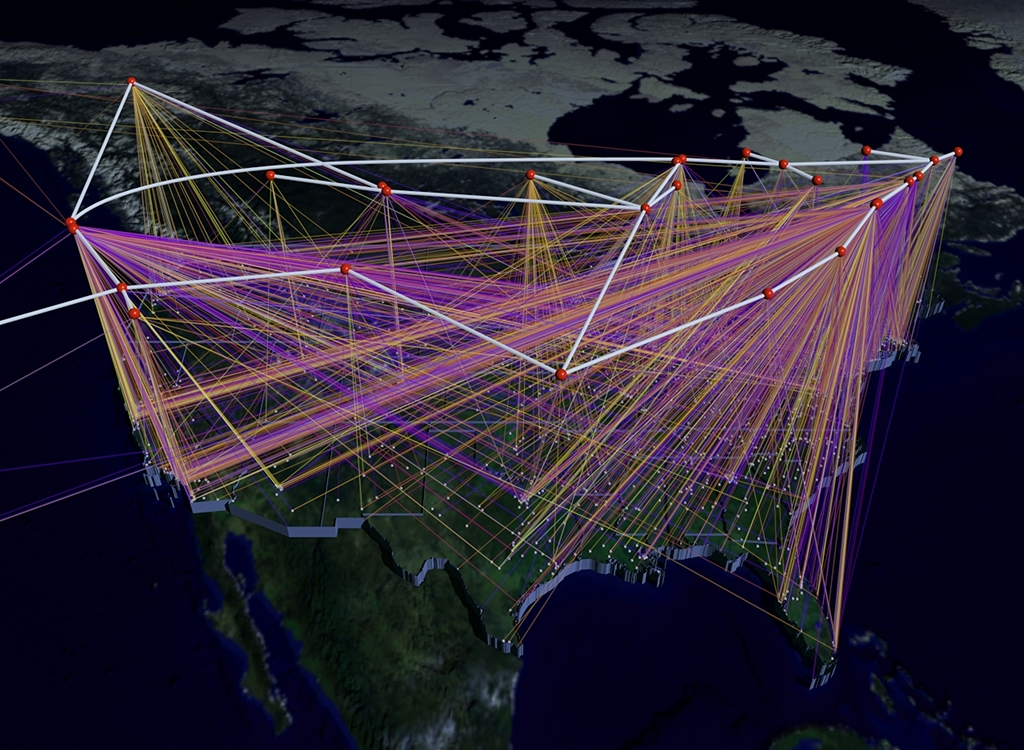
\includegraphics[height=4cm]{pic/01-internet.jpg}
				\caption{Internet一部分的可视化}
			\end{minipage}
		\end{figure}
		
		
	\section{网络的图表示}
		要研究各种不同的复杂网络在结构上的共性,首先需要一种描述网络的统一的工具。这个工具就是图。\par
		一个具体网络可以抽象为一个由点集$V$和边集$E$组成的图$G=(V,E)$。节点数记为$N=|V|$,边数记为$M=|E|$。 一条边对应一对点。\par
		
		\subsection{七桥问题}
			实际网络的图表示方法可以追溯到18世纪伟大的数学家欧拉(Euler)对著名的“Kinigsberg七桥问题”的研究。七桥问题可以见下图:
			
			\begin{figure}[htbp]
				\centering
				%\flushleft
				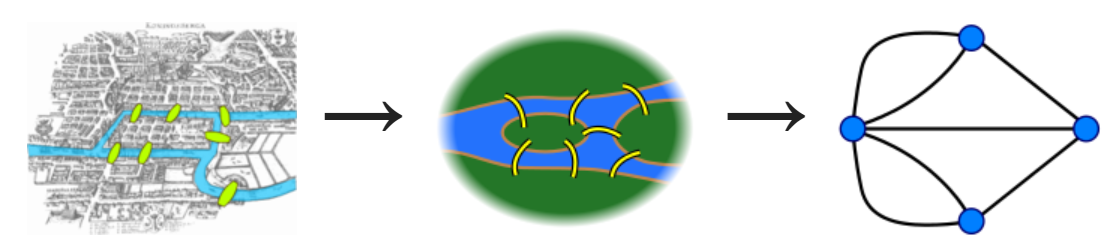
\includegraphics[width=0.7\textwidth]{pic/01-sevenb.png}
				\caption{七桥问题-Euler图}
				\label{003}
			\end{figure}
			
			Kinigsberg是东普鲁士(现俄罗斯)的一个城镇,城中有一条横贯城区的河流,河中有两个岛,两岸和两岛之间共架有7座桥,一个人能否在一次散步中走过所有的七座桥并且每座桥都只经过一次,最后返回原地呢? \par
			欧拉把这个问题抽象成抽象成由4个点和7条线构成的一个图,并且将问题等价为能否一笔画成这个图的问题。能够一笔画成的图形,一定只有一个起点和终点,这里还要求起点和终点重合,那么中间经过的每一个点总是包含进去的一条线和出来的一条线,这样出去起点和终点外,每一条都只能有偶数条线与之相连。因此,如果要求起点和终点重合的话,那么能够一笔画出的图形中所有的点都必然有偶数条线与之相连。而从图~\ref{003}来看,每个点都是有3条或5条线通过,所以不能一笔画出这个图形。所以七桥问题是没有解的。\par
			欧拉对七桥问题的抽象和论证思想,开创了数学中的一个分支——图论(graph theory)的研究。因此,欧拉被公认为图论之父,而图~\ref{003}也被称为欧拉图。事实上,今天人们关于复杂网络的研究与欧拉当年关于七桥问题的研究在某种程度上是一脉相承的,即网络结构与网络性质密切相关。
	
		
		\subsection{三个基本概念}
			在刻复杂网络结构的统计特性上,人们提出了很多概念和方法,其中有三个基本的概念:平均路径长度(average path length)、聚类系数(clustering coefficient)和度分布(degree distribution)。\par
			根据上文的网络的图表示,根据边是否有方向,有无向网络和有向网络的划分。如果每条边都有相应的权重,那么这个网络就是加权网络,否则就是无权网络。一个网络中的节点也有可能多种多样。重边是指两个点之间多于一条边,自环是指有边的起点和终点是同一个点。在图论中,没有重边和自环的点称为简单图(simple graph),我们所研究的大部分图都是简单图。
			
		
		\subsubsection*{平均路径长度}
				网络中两个节点$i$和$j$之间的距离$d_{ij}$定义为连接这两个节点的最短路径上的边数。网络中任意两个节点之间额距离的最大值称为网络的直径(diameter),记为$D$,即
				$$D = \max\limits_{i,j}d_{ij}$$ \par
				网络的平均路径长度$L$定义为任意两个节点之间的距离的平均值,即
				$$L = \frac{1}{2} \frac{1}{N(N+1)}\sum\limits_{i \ge j}d_{ij}$$ 
				其中$N$是网络节点数。网络的平均路径长度也称为网络的特征路径长度(characteristic path length)。
		
		\subsubsection*{聚类系数}	
			在你的朋友关系网络中,你的两个朋友很有可能彼此也是朋友,这种属性称为网络的聚类特性。\par
			一般地,假设网络中的一个节点$i$有$k_i$条边将它和其他节点相连,这$k_i$个节点就称为节点$i$的邻居。显然,$k_i$个节点间最多有$k_i(k_i-1)/2$条边。而这$k_i$个节点之间实际存在的b边数$E_i$和总的可能的边数之比就定义为节点$i$的聚类系数$C_i$,即
				$$ C_i = 2E_i / k_i (k_i - 1)$$
			从几何特性上看,上式可等价为
			$$C_i = \frac{\text{与点}i\text{相连的三角形的数量} }{\text{与点}i\text{相连的三元组的数量}}$$	
			其中,与节点$i$相连的三元组是指包括节点$i$的三个节点,并且至少存在从节点$i$到其他两个节点的两条边。
			
			\begin{figure}[htbp]
				\centering
				%\flushleft
			 	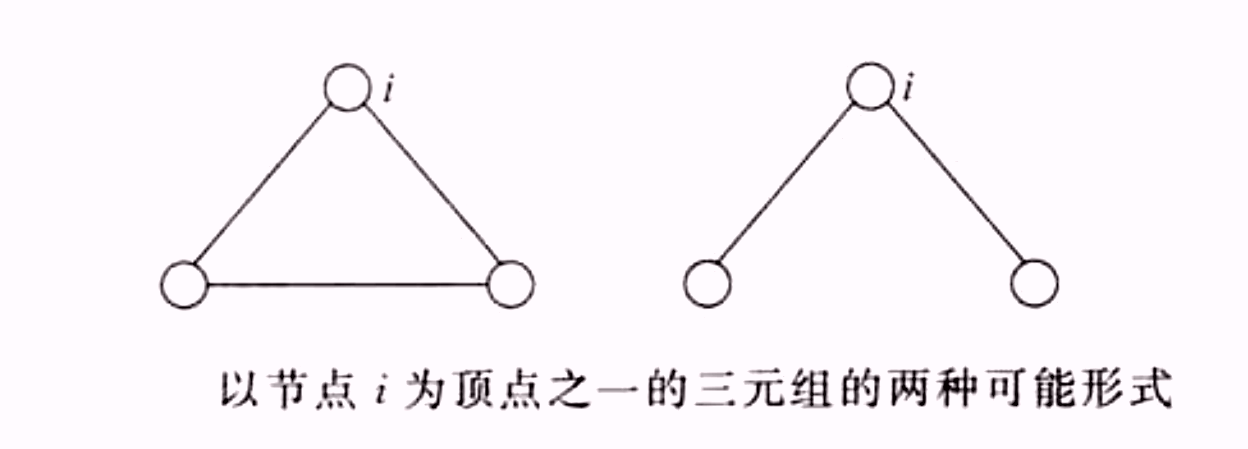
\includegraphics[width=0.8\textwidth]{pic/01-three.png}
				\caption{以节点$i$为顶点之一的三元组的两种可能}
			\end{figure}
			\par
			整个网络的聚类系数$C$就是所有节点$i$的聚类系数$C_i$的平均值。很明显,$C=0$当且仅当所有的节点均为孤立节点,即没有任何连接边;$C=1$当且仅当网络是全局耦合的,即网络中任意两个节点都直接相连。对于一个含有$N$个节点的完全随机的网络,当$N$很大时,$C=O(N^{-1})$。而许多大规模的实际网络都具有很明显的聚类效应,它们的聚类系数尽管远小于1但却比$O(N^{-1})$要大很多。
			
		\subsubsection*{度与度分布}	
			度(degree)是单独节点的属性中简单而又重要的概念。节点$i$的度定义为与该节点连接的其他节点的数目。有向网络中一个节点的度又分为出度(out-degree)和入度(in-degree)。度越大从某种意义上意味着该节点越重要。 \par
			所有节点$i$的度$k_i$的期望称为网络的(节点)平均度,记为$<k>$。网络中节点的度分布可用分布函数$P(k)$来描述。$P(k)$表示的是一个随机选定的节点的度恰好为$k$的概率。\par
			完全随机网络的度分布近似Poisson分布。很多实际网络,如社交网络的度分布近似幂律分布~\cite{w1_book}。
			
			\begin{figure}[htbp]
				\centering
				%\flushleft
				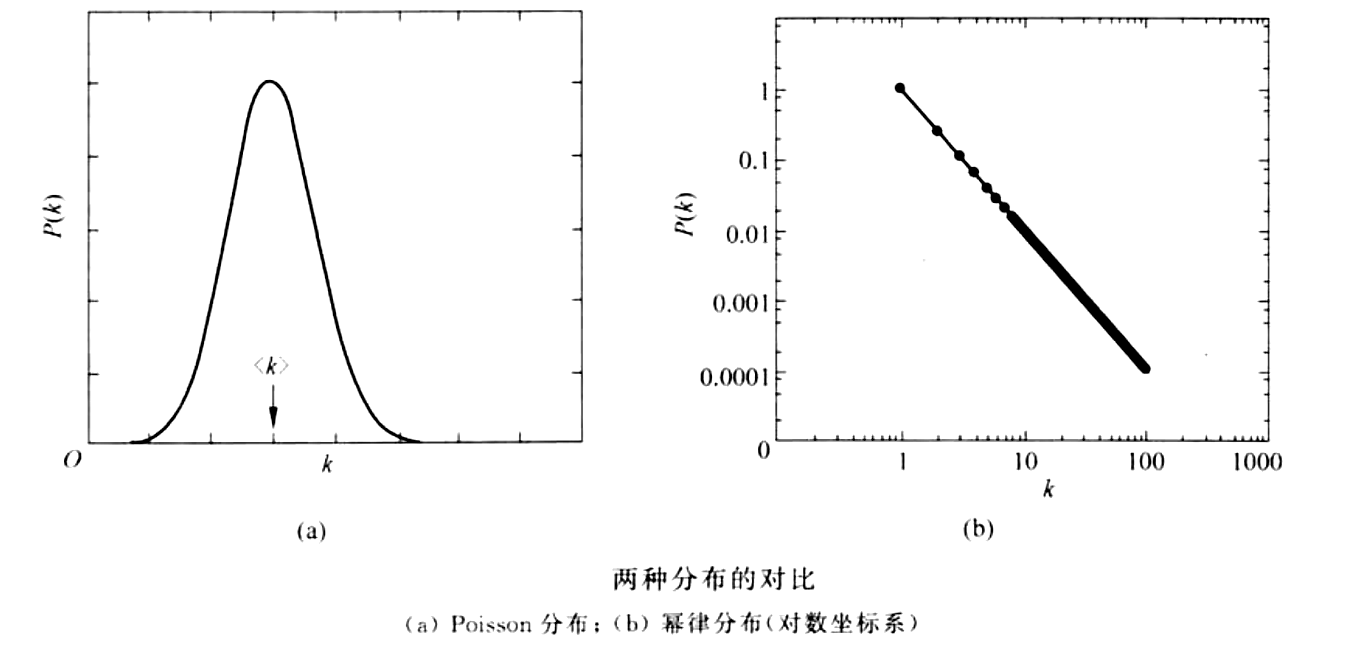
\includegraphics[width=0.8\textwidth]{pic/01-pandp.png}
				\caption{Poisson分布和幂律分布}
			\end{figure}
			
			幂律分布也称为无标度分布(scale-free)分布,具有幂律分布的网络也称为无标度网络,这是因为幂律分布函数具有无标度性质:考虑一个概率分布函数$f(x)$,如果对任意给定常数$a$,存在常数$b$使得函数$f(x)$满足如下“无标度条件”。
			$$f(ax) = bf(x)$$
			那么必有(假定$f(1)f^\prime(1) \ne 0$)
			$$f(x) = f(1)x^{-\gamma}, \gamma = -f(1)f^\prime(1)$$
			证明可由带入$x=1$然后得到常数$b$,再将$b$的值代回解微分方程可得。\par
			这个结果也就是说,幂律分布函数是唯一满足“无标度条件”的概率分布函数。 \par
			度分布满足Poisson分布的网络度大都集中在某个标度附近,称之为均匀网络;度分布满足幂律分布的网络绝大部分节点度很低,但少量的节点度非常高,称为非均匀网络。
			
\section{复杂网络案例研究}
		
	\subsection{规则网络}
		常见的规则网络有全局耦合(coupled)网络,最近邻耦合网络,星形耦合网络。\par
		全局耦合网络:任意两点均有边相连。具有最小的平均路径长度$L_{gc}=1$,最大的聚类系数$C_{gc}=1$。大多数大型实际网络都是很稀疏的。\par
		最近邻耦合网络: 每个节点只和周围的邻居节点相连。	具有周期边界条件的最近邻耦合网络,$N$个点围成一个环,每个节点与左右$K/2$个点相连,$K$是偶数。对较大的$K$值,聚类系数$C_{nc}=\frac{3(K-2)}{4(K-1)}\approx\frac{3}{4}$,平均路径长度$L_{nc}\approx \frac{N}{2K} \rightarrow \infty ((N \rightarrow \infty)$。\par
		星形耦合网络:有一个中心点,其余$N-1$个点只与中心点相连。聚类系数$C_{star}=\frac{N-1}{N} \rightarrow (N \rightarrow \infty)$,平均路径长度$L_{star}=2- \frac{2(N-1)}{N(N-1)} \rightarrow 2 (N \rightarrow \infty)$。
		
		\begin{figure}[htbp]
			\centering
			%\flushleft
			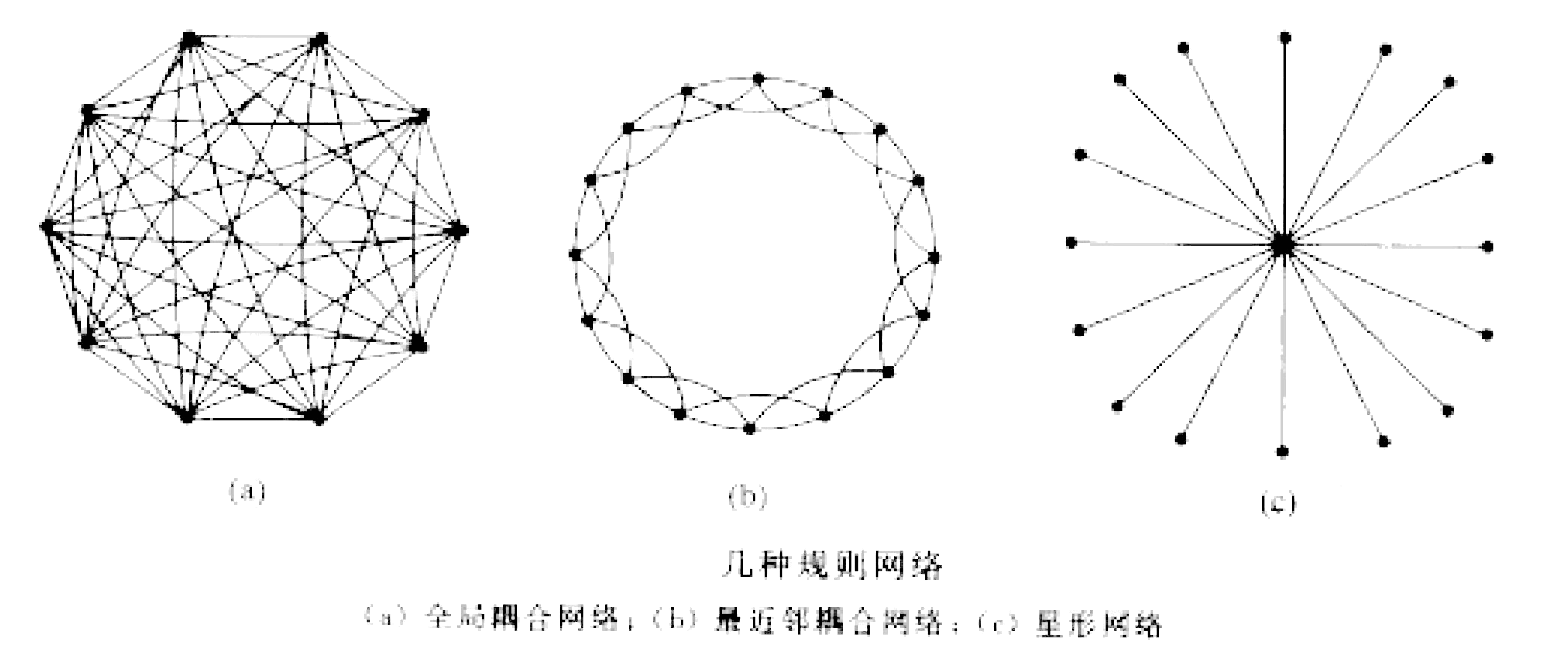
\includegraphics[width=0.8\textwidth]{pic/01-rgraph.png}
			\caption{全局耦合网络、最近邻耦合网络、星形耦合网络}
		\end{figure}
		
	\subsection{随机网络}	
		与完全规则网络相反的是完全随机网络。其中一个典型的模型是ER随机网络(Erdős–Rényi model,1959)。\par
		
		\begin{figure}[htbp]
			\centering
			%\flushleft
			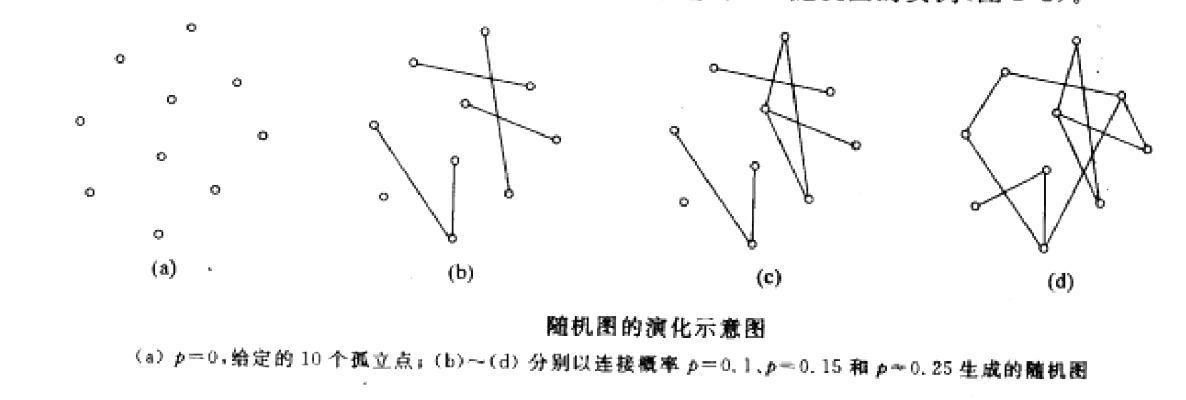
\includegraphics[width=0.7\textwidth]{pic/01-ERgraph.png}
			\caption{ER随机图模型}
		\end{figure}
		假设存在$N(\gg 1)$个点,以概率$p$在两个点之间连线构成的图,就叫做ER随机图模型。随机图理论的一个主要的研究课题是:当$p$不同时,随机图会产生哪些特殊的属性?限于篇幅,不再讲述,在~\cite{w1_book}中随机网络一章,作者有详细阐述,感兴趣的读者可以自行查阅。\par
		ER随机图的平均度是$<k> = p(N-1) \approx pN$,由二项分布$\rightarrow $泊松分布($N\rightarrow \infty$)。因此,ER随机图也称为“Poission随机图”。\par
		平均路径长度为网络规模的对数增长函数,$L_{ER} \propto \ln N / \ln <k>$(小世界特性)。这种平均路径长度为网络规模的对数增长函数的特性就是典型的小世界特征。因为$\ln N$增长得很慢,这就使得即使是规模很大的网络也可以具有很小的平均路径长度。\par
		ER随机图的聚类系数$C=p=<k>/N \ll 1$。 这意味着大规模的稀疏ER随机图没有聚类特性。而现实中的复杂网络一般都具有明显的聚类特性。\par
		随机网络与实际复杂网络模型相比存在明显缺陷。
		

	\subsection{小世界网络}
		小世界网络是指具有较短平均路径长度的同时,又具有较高的聚类系数的一类网络。\par
		
		\subsubsection*{WS小世界模型}
		作为从完全规则网络向完全随机图的过渡,WS小世界模型(Watts \& Strogtz,1998)~\cite{paper_02}被引入。WS小世界模型的构造算法如下:
		
		\begin{center}
		\fbox{
			\centering
			\parbox[tc][100pt][t]{400pt}{
				\textbf{WS小世界模型}
				\begin{enumerate}[(1)]
					\item 从规则图开始:考虑一个含有$N$个点的环形最近邻耦合网络,每个节点与左右相邻的$K/2$个节点相连,$K$是偶数。
					\item 随机化重连:以概率$p$随机的重新连接网络中的每条边,即边的一个端点保持不变,另一个节点在网络中随机选取。约定没有重边和自环。
				\end{enumerate}
		}} 
		\end{center}
	
		$p=0$时,对应完全规则网络;$p=1$时,对应完全随机网络,通过调节$p$值就可以控制从完全规则网络到完全随机网络的过度。\par
		由上诉算法得到的网络模型的聚类系数$C(p)$和平均路径长度$L(p)$的特性,都可以看做是重连概率$p$的的函数。一个完全规则最近邻耦合网络是高度聚类但平均路径长度很大。当$p$较小时,新的网络与原始网络局部属性差别不大,从而网络的聚类系数变化也不大,平均路径长度却下降很快。从而具有小世界网络的性质。
		
		\subsubsection*{NW小世界模型}
		WS小世界网络构造算法中的随机化过程有可能破坏网络的连通性。由此提出了NW小世界模型(Newman \& Watts,2000)~\cite{paper_03} :
		\begin{center}
			\fbox{
				\centering
				\parbox[tc][100pt][t]{400pt}{
					\textbf{NW小世界模型}
					\begin{enumerate}[(1)]
						\item 从规则图开始:考虑一个含有$N$个点的环形最近邻耦合网络,每个节点与左右相邻的$K/2$个节点相连,$K$是偶数。
						\item 随机化加边:以概率$p$在在随机选取的一对节点之间加上一条边。任意两各节点之间至多有一条边,约定没有重边和自环。
					\end{enumerate}
			}}
		\end{center}
		小世界网络反映了朋友关系网络的一些特性,大部分人的朋友都是其邻居或单位同事,但也有一些人住得很远。
		
		\subsubsection*{统计性质}
		下面介绍小世界网络模型的一些统计性质:
		\begin{enumerate}[1.]
			\item 聚类系数 \par
					WS小世界网络:$C(p) = \frac{3(K-2)}{4(K-1)}(1-p)^3$ \\
					NW小世界网络:$C(p) = \frac{3(K-2)}{4(K-1) + 4Kp(p+2)}$ 
			\item 平均路径长度 \par
					没有精确的显示表达式,但有一些近似表达式。可以近似的认为,$p、K$确定的情况下,$L(p) \propto \ln N$。
			\item	度分布 \par
					大体上满足二项分布,极限情况下逼近泊松分布,是所有节点的度都大致相等的均匀网络。
		\end{enumerate} \par
		有一些利用小波分析进行小世界网络分析的研究,可以参见~\cite{w1_book}第二章。 \par
		现实生活中有很多小世界网络的例子,如六度分离理论:世界上任何互不相识的两人,只需要很少的中间人就能够建立起联系。还有一些关于小世界网络的有趣实验,Kevin Bacon游戏和Erdős数等等。 
		
		
	\subsection{无标度网络}
		ER随机图和WS小世界模型的度分布可近似用Poisson分布表示(称为均匀网络或指数网络),大部分节点的度集中在某个特征长度附近。然而许多实际复杂网络(Internet、新陈代谢网络)的度分布具有幂律形式,这类网络节点的连接度没有明显的特征长度,故称为无标度网络。\par
		
		为了解释幂律分布的产生机理,提出了BA模型~\cite{paper_04}。他们认为许多网络模型都没有考虑到实际网络的以下两个重要特性:
		\begin{itemize}
			\item 增长特性:网络规模是不断扩大。例如每个月都会有大量的科研文章发表,WWW上每天都会产生大量新的网页。 
			\item 优先连接:新的节点趋向于与那些具有较高连接度的节点相连接。称为“富者更富”或者“马太效应”。例如新发表的文章更倾向于引用一些已经被广泛引用的重要文献。
		\end{itemize}
	
		\subsubsection*{BA无标度网络}
			BA无标度网络~\cite{paper_06}的构造算法如下:
			\begin{center}	
				\fbox{
					\centering
					\parbox[tc][144pt][t]{400pt}{
						\textbf{BA无标度模型构造算法}
						\begin{enumerate}[(1)]
							\item 增长:从一个具有$m_0$个节点的网络开始,每次引入一个新的节点连接到$m$个已存在的节点上,$m\le m_0$。
							\item 优先连接:一个新节点与一个已经存在的节点$i$相连接的概率$\prod_i$与节点$i$的度$k_i$、节点$j$的度$k_j$之间满足如下关系:
							$$\prod_i = \frac{k_i}{\sum\limits_{j}k_j}$$
						\end{enumerate}
					}
				}
			\end{center}
	
			\begin{figure}[htbp]
				\centering
				%\flushleft
				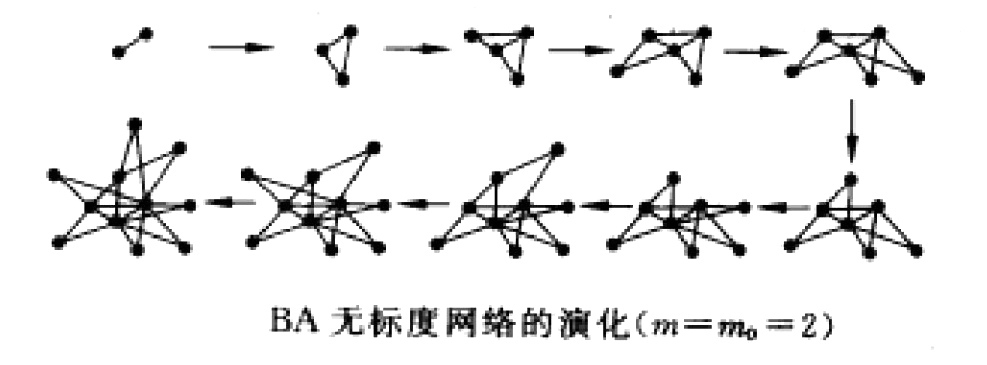
\includegraphics[width=0.7\textwidth]{pic/01-BA.png}
				\caption{BA无标度网络的演化($m=m_0=2$)}
			\end{figure}
			\par
			BA无标度网络的平均路径长度: $L \propto \frac{\log N}{\log \log N}$,这表明该网络也具有小世界特性。 当网络规模充分大的时候,BA无标度网络没有明显的聚类特征。BA无标度网络的度分可近似看作幂律分布。\par

			因为无标度网络的度分布满足幂律分布,在随机移走少量节点时,绝大部分节点仍是连通的,这体现了无标度网络的鲁棒性;然而,如果针对性的移走无标度网络中那些具有很高的度分布的节点,只需要移除少部分可能无标度网络的连通性就会被破坏,这又体现了无标度网络的鲁棒性。
			
			
			\subsubsection*{适应度模型}
				BA无标度网络中,越老的节点具有越高的度。实际网络中并非如此,有些节点由于自身的特殊性质,更容易被新新加入的节点所连接。如个人的交友能力和科研论文的质量等等。因此~\cite{paper_05}提出了适应度模型:\par
				
				\begin{center}	
					\fbox{
						\centering
						\parbox[tc][144pt][t]{400pt}{
							\textbf{适应度模型构造算法}
							\begin{enumerate}[(1)]
								\item 增长:从一个具有$m_0$个节点的网络开始,每次引入一个新的节点连接到$m$个已存在的节点上,$m\le m_0$。每个节点的适应度按概率分布$\rho(\eta)$选取。
								\item 优先连接:一个新节点与一个已经存在的节点$i$相连接的概率$\prod_i$与节点$i$的度$k_i$、节点$j$的度$k_j$和适应度$\eta_i$之间满足如下关系:
								$$\prod_i = \frac{\eta_i k_i}{\sum\limits_{j}\eta_i k_j}$$
							\end{enumerate}
					}}
				\end{center} \par
				适应度模型中,假如年轻的节点具有较高的适应度,在后续演化过程中会获得更多的边。\par
				适应度分布的性质不同,适应度模型会有不同的行为表现。
				
	\subsection{自相似性、自组织与吸引子}
	
		\subsubsection*{自相似性}
			局部在某种意义上与整体相似,就是自相似性,是分形的基本特征。实际中很多复杂网络也具有自相似性。\par
			
			\begin{figure}[htbp]
				\centering
				%\flushleft
				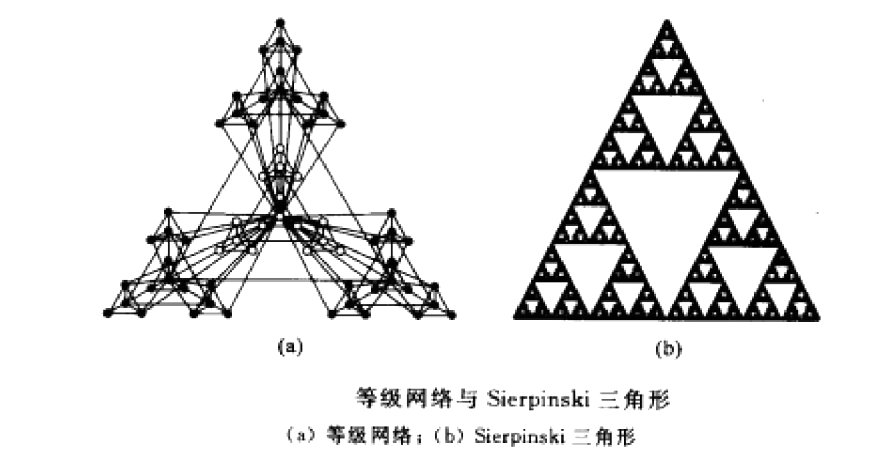
\includegraphics[width=0.75\textwidth]{pic/01-self.png}
				\caption{等级网络和Sierpinski三角形}
			\end{figure}
			
			与自相似性密切相关的一个概念是分数维,计算自相似分形的维数的一种常用的方法是盒计数法。任意一个几何推行都可以嵌入在一个整数维的欧式空间之中,用边长$l_B$的盒子来完全覆盖一个几何图形,需要的最少盒子数为$N_B(l_B)$。图形的维数近似计算公式为:
				$$d_B \approx - \frac{\ln N_B(l_B)}{ln(l_N)} (l_B \rightarrow 0)$$
			一般情况下,当盒子尺寸$l_B$趋于零时,才可以由上式得到维数的精确值。\par
			盒计数法存在的问题是分割方式难以寻找。
		
		\subsubsection*{自组织}
			自我组织,也称为自组织。自组织是一系统内部组织化的过程,通常是一开放系统,在没有外部来源引导或管理之下会自行增加其复杂性。 自组织是从最初的无序系统中各部分之间的局部相互作用,产生某种全局有序或协调的形式的一种过程。这种过程是自发产生的,它不由任何中介或系统内部或外部的子系统所主导或控制。
			
		\subsubsection*{吸引子}
			一个系统有朝某个稳态发展的趋势,这个稳态就叫做吸引子。吸引子分为平庸吸引子和奇异吸引子。\par
			例如如钟摆系统有一个平庸吸引子,其使钟摆系统向停止晃动的稳态发展。\par
			平庸吸引子有不动点(平衡)、极限环(周期运动)和整数维环面(概周期运动)三种模式。而不属于平庸的吸引子的都称为奇异吸引子,它表现了混沌系统中非周期性,无序的系统状态,例如天气系统。\par
			对于吸引子,学术上并没有完善的定义,目前仅处于概念阶段。
			
\section{总结}
	本文只是简单介绍了下复杂网络的研究基础。实际上,复杂网络是就像他的名字一样,是一门十分复杂的学科,许多复杂网络中存在的现象至今还没有明确的解释并且正在研究之中。要搞清楚复杂网络,是一个非常浩大的工程。有兴趣的读者可以自行查阅文献或者动手实验。
			
			
	
% bibe
\bibliographystyle{plain}
\bibliography{refs}		
\end{document}


